\chapter{Applicazioni astrofisiche}
\label{chap:applicazioni}

\section{Il sistema binario Sgr~A*~-~S2}
\label{sec:sgra}

La terza legge di Keplero permette di determinare la massa di un corpo celeste
se sono noti i parametri orbitali e la massa di un altro corpo con cui
costituisce un sistema binario.

\begin{figure}
  \centering
  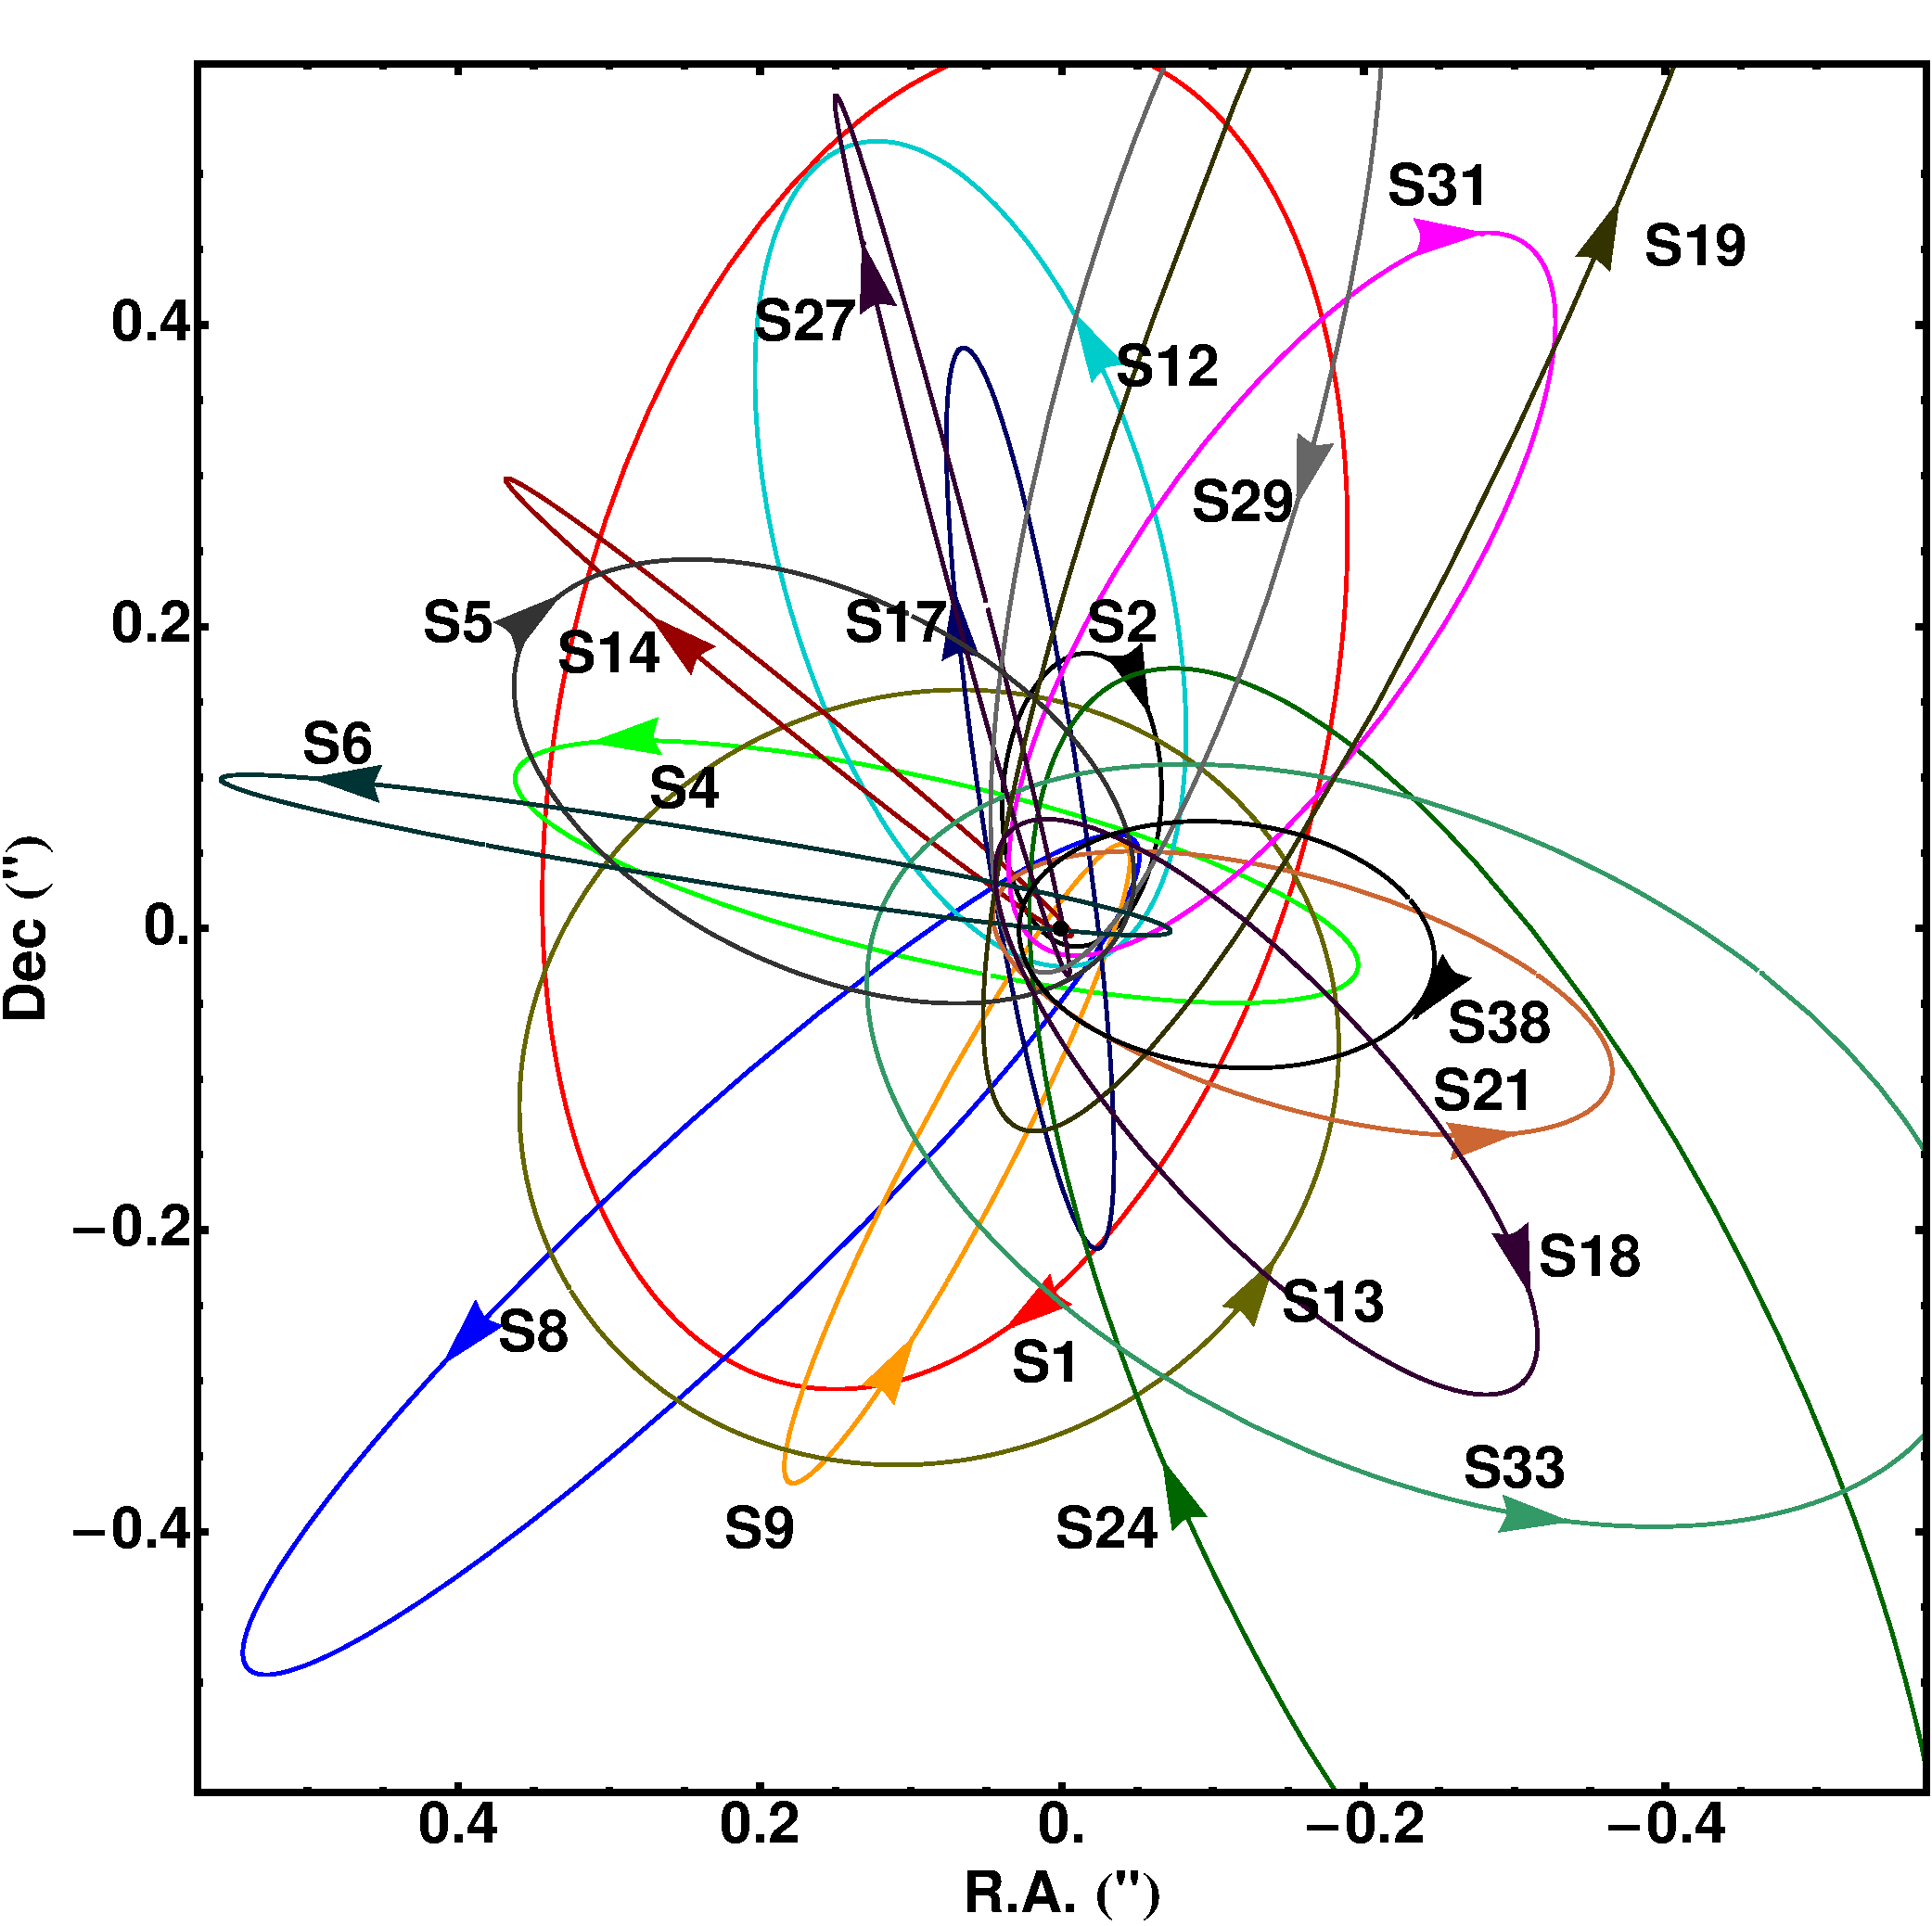
\includegraphics[width=7cm]{Immagini/orbite_sgra}
  \caption[Orbite di alcune delle stelle che intorno al buco nero
  Sgr~A*]{Rappresentazione delle orbite di alcune delle stelle che orbitano
    intorno al buco nero. La figura, tratta da \textcite{2009ApJ...692.1075G}, è
    centrata in Sgr~A*}
  \label{fig:orbite-sgra}
\end{figure}
Si suppone che la regione Sagittarius~A* (Sgr~A*), nel centro della nostra
galassia, sia sede di un buco nero supermassivo, cioè con una massa oltre $10^6$
volte più grande di quella del Sole. Intorno a questo buco nero orbitano
numerose stelle e le orbite di alcune di esse possono essere osservate nella
Figura~\ref{fig:orbite-sgra}. La stella più importante per i nostri scopi è S2
(chiamata a volte S0-2 e di massa circa \SI{15}{\solarmass}), poiché fra le
stelle che orbitano intorno al buco nero è quella che ha il più breve periodo di
rivoluzione, pari a circa $15$ anni, e fra le stelle di questa regione a breve
periodo è la più luminosa, quindi più facile da individuare. Le osservazioni
astronomiche di S2 sono cominciate nel 1992 e da pochi anni ha completato
un'intera rivoluzione a partire da quella data, quindi è una ricca fonte di
informazioni per lo studio del buco nero. L'orbita di S2 intorno al buco nero
può essere considerata con buona approssimazione kepleriana quindi possiamo
utilizzare la~\eqref{eq:terza-legge-keplero} per stimare la massa
$M_\textup{BH}$ del buco nero. \textcite{2008ApJ...689.1044G} hanno studiato il
moto di S2 ricavando i dati riportati nella
Tabella~\ref{tab:parametri-orbitali-S2}.
\begin{table}
  \centering
  \caption[Parametri orbitali della stella S2]{Parametri orbitali della stella
    S2. $R_0$ è la distanza dalla Terra, $P$ è il periodo di rivoluzione, $a$
    è il semiasse maggiore dell'orbita ed $e$ la sua eccentricità,
    $R_\textup{min}$ è la distanza di periapside e $M_{\textup{S}2}$ è la
    massa della stella}
  \label{tab:parametri-orbitali-S2}
  \begin{tabular}{lc}
    \toprule
    Grandezza & Valore \\
    \midrule
    $R_0$ & \SI{7.96}{\kilo\parsec} \\
    $P$ & \SI{15.86}{\year} \\
    $a$ & \SI{126.5}{\milli\arcsecond} \\
    $e$ & $0.8970$ \\
    $R_\textup{min}$ & \SI{0.535}{\milli\parsec} \\
    $M_{\textup{S}2}$ & circa \SI{15}{\solarmass} \\
    \bottomrule
  \end{tabular}
\end{table}
Il semiasse maggiore dell'orbita è espresso in millesimi di arcosecondo, questo
valore può essere convertito in parsec, conoscendo la distanza $R_0$ della Terra
dal corpo, con la seguente relazione
\begin{equation}
  a [\si{\parsec}] = \frac{a [\si{\arcsecond}] \cdot R_0 [\si{\parsec}] \cdot
    \pi}{3600 \cdot 180} = \SI{4.88e-3}{\parsec}.
\end{equation}
Poiché $M_\textup{BH}$ è sicuramente molto più grande di $M_{\textup{S}2}$
possiamo porre $M_\textup{T} \approx M_\textup{BH}$
nella~\ref{eq:terza-legge-keplero} e otteniamo
\begin{equation}
  M_\textup{BH} \approx M_\textup{T} = \frac{4\pi^2a^3}{GP^2} =
  \SI{4.06e6}{\solarmass}.
\end{equation}
In realtà quella calcolata non è esattamente la massa del buco nero ma tutta la
massa che, nel piano dell'orbita di S2, è contenuta nella circonferenza di
raggio $R_\textup{min}$ e centro nel fuoco. Metodi più elaborati per la stima
della massa del buco nero possono essere trovati in
\textcite{2008ApJ...689.1044G} e \textcite{2009ApJ...692.1075G}.

Gli astronomi continuano a studiare il moto di S2 poiché sperano di osservare
delle deviazioni dall'orbita puramente kepleriana previste dalla teoria della
relatività le quali permetterebbero di effettuare una diversa stima della massa
del buco nero.

\section{I pianeti extrasolari}
\label{sec:extrasolari}

Molti pianeti extrasolari costituiscono, almeno in prima approssimazione, un
sistema binario insieme alla stella intorno alla quale orbitano e dallo studio
delle eclissi della stella dietro al pianeta è possibile ricavare delle
caratteristiche dei due corpi. Qui ci limiteremo a studiare alcune proprietà del
fenomeno dell'eclissi.

Vediamo sotto quali condizioni è possibile per un osservatore esterno vedere
un'eclissi della stella dietro al pianeta studiato. Per semplicità assumiamo che
le orbite dei due corpi siano circolari, quindi $e \approx 0$, che questi siano
perfettamente sferici e che possano essere trascurati gli effetti dovuti
all'atmosfera. Con riferimento alla Figura % TODO: creare figura, scrivere
                                % didascalia che faccia riferimento al fatto che
                                % il piano in cui si svolgono le orbite dei due
                                % corpi è ortogonale al piano della figura e
                                % inserire riferimento nel testo
il corpo di massa $m_1$ è la stella, di raggio $r_\star$, e quello di massa
$m_2$ è il pianeta, il cui raggio è $r$. La distanza reciproca fra i centri dei
due corpi vale $a$. Se indichiamo con $i \in \mathopen{[}0, \pi/2\mathclose{]}$
l'angolo di inclinazione sotto il quale l'osservatore vede il sistema, l'angolo
minimo che permette all'osservatore di assistere a un'eclissi è quello
rappresentato nella figura, cioè con l'asse $x''$ passante per il centro della
stella e tangente alla superficie del pianeta. Dunque
\begin{equation}
  \cos(\pi/2 - i) = \frac{\sqrt{a^2 - r^2}}{a} = \sqrt{1 - \frac{r^2}{a^2}}.
\end{equation}
Generalmente si ha $a \gg r_\star \gg r$, quindi $\cos(\pi/2 - i) \approx 1$,
cioè $i \approx \pi/2$.

Nella Figura % TODO: creare figura, scrivere didascalia descrittiva che faccia
             % riferimento anche alla curva di luminosità e inserire riferimento
è rappresentata una schematizzazione di un'eclissi della stella, nel caso in cui
$i = \pi/2$. L'osservatore è fisso davanti alla stella e vede il pianeta che le
passa davanti, in vari istanti. Quando il pianeta non copre la stella la
luminosità del sistema è massima, quando inizia a nasconderla parzialmente
(istante di \emph{ingresso iniziale}, $t_{\textup{ii}}$) la luminosità decresce
fino a raggiungere un minimo nell'istante in cui si trova completamente davanti
alla stella (\emph{ingresso finale}, $t_{\textup{if}}$). La luminosità rimane
minima per tutto il tempo in cui il pianeta si trova davanti alla stella,
successivamente aumenta quando il pianeta esce parzialmente dalla stella
(\emph{egresso iniziale}, $t_{\textup{ei}}$) e ritorna massima non appena il
pianeta non copre più la stella (\emph{egresso finale}, $t_{\textup{ef}}$). Gli
istanti fin qui definiti sono detti \emph{punti di contatto}. Esistono poi i
\emph{punti di mezzo ingresso} che sono quelli in cui la curva di luminosità
raggiunge il valore intermedio fra il massimo e il minimo. In particolare
abbiamo il \emph{mezzo ingresso iniziale} ($t_{\textup{mi}}$) quando la
luminosità sta diminuendo e il \emph{mezzo ingresso finale} ($t_{\textup{mf}}$)
quando la luminosità ricomincia ad aumentare. Definiamo la
\emph{durata dell'eclissi} $\Delta t$ come il tempo che intercorre fra
l'ingresso iniziale e l'egresso finale:
$\Delta t = t_{\textup{ef}} - t_{\textup{ii}}$. La velocità di rivoluzione del
pianeta intorno alla stella è $P/(2\pi a)$, avendo indicato con $P$ il periodo
di rivoluzione del pianeta intorno alla stella, e, sempre nell'approssimazione
$a \gg r_\star \gg r$, lo spazio percorso dal pianeta fra gli istanti
$t_{\textup{ii}}$ e $t_{\textup{ef}}$ è $2(r_\star + r)$. Allora la durata
dell'eclissi è
\begin{equation}
  \Delta t \approx \frac{P}{2\pi a}2(r_\star + r) = \frac{P(r_\star + r)}{\pi
    a}.
\end{equation}

Se l'angolo di inclinazione $i$ non vale esattamente $\pi/2$, anche, come
abbiamo visto, per poter osservare un'eclissi deve comunque aversi $i \approx
\pi/2$, l'osservatore non vede il pianeta passare esattamente davanti
all'equatore della stella ma leggermente più spostato, come nella Figura % TODO:
                                % inserire figura e riferimento.
. Per calcolare lo spostamento apparente del pianeta rispetto all'equatore si
può vedere la Figura. % TODO: inserire figura e riferimento (se riesci puoi
                      % mettere questa figura e la precedente insieme).
Da semplici calcoli trigonometrici si ricava che lo spostamento apparente vale
$a \cos i$. Le definizioni dei punti di contatto e di mezzo ingresso valgono
anche per questo caso. Osservando la Figura % TODO: inserire riferimento
                                % all'ultima figura
si ricava, sempre usando la trigonometria, che lo spazio percorso dal pianeta
fra gli istanti $t_{\textup{ii}}$ e $t_{\textup{ef}}$ è $2(r_\star + r)$ è circa
$2\sqrt{(r_\star + r)^2 - a^2\cos^2 i}$, quindi la durata dell'eclissi in questo
caso è
\begin{equation}
  \Delta t \approx \frac{P}{2\pi a} 2\sqrt{(r_\star + r)^2 - a^2\cos^2 i} =
  \frac{P}{\pi} \sqrt{\left(\frac{r_\star + r}{a}\right)^2 - \cos^2 i}.
\end{equation}
Per $i = \pi/2$ si riottiene il risultato precedente.

Calcoliamo l'area del disco della stella coperta dal pianeta durante
l'eclissi. La distanza che prenderemo in considerazione non sarà la distanza
reale $a$ fra i due corpi ma quella proiettata $d$ nel piano del cielo
dell'osservatore e introdotta nel paragrafo~\ref{sec:geometria-sistema}. Se in
un certo istante di tempo si ha $d > r_\star + r$, i due corpi non sono
sovrapposti nel cielo dell'osservatore quindi non si sta verificando
l'eclissi. Se invece $d \leq r_\star + r$ il pianeta copre parzialmente la
stella. Finché $\sqrt{r_\star^2 - r^2} \leq d \leq r_\star + r$, l'area di
sovrapposizione è la somma delle due aree $S_1$ e $S_2$ della
Figura. % TODO: creare figura e inserire riferimento
Per il teorema del coseno, l'angolo $\theta_1$ % TODO: nella figura indicare,
                                % correttamente, gli angoli \theta_1 e
                                % \theta_2. Dopo aver messo la figura
                                % ricontrollare tutte le formule seguenti, per
                                % vedere se ho indovinato i nomi degli angoli.
è dato da
\begin{equation}
  \theta_1 = 2 \arccos \frac{r_\star^2 - r^2 + d^2}{2r_\star d}
\end{equation}
e analogamente per l'angolo $\theta_2$ abbiamo
\begin{equation}
  \theta_2 = 2 \arccos \frac{r^2 - r_\star^2 + d^2}{2rd}.
\end{equation}
Le aree $S_1$ e $S_2$ valgono rispettivamente
\begin{subequations}
  \begin{align}
    S_1 &= \frac{\theta_2}{2\pi}\pi r^2 - \frac{r^2}{2}\sin\theta_2 =
    \frac{r^2}{2}(\theta_2 - \sin\theta_2), \\
    S_2 &= \frac{\theta_1}{2\pi}\pi r_\star^2 - \frac{r_\star^2}{2}\sin\theta_1
    = \frac{r_\star^2}{2}(\theta_1 - \sin\theta_1).
  \end{align}
\end{subequations}
Dunque in questo caso l'area di sovrapposizione $\delta A$ vale
\begin{equation}
  \delta A = S_1 + S_2 = \frac{r_\star^2}{2}(\theta_1 - \sin\theta_1) +
  \frac{r^2}{2}(\theta_2 - \sin\theta_2).
\end{equation}
Se $r_\star - r \leq d < \sqrt{r_\star^2 - r^2}$ risulta $\theta_2 > \pi$,
quindi $S_2$ è la somma del settore circolare di angolo $\theta_2$ e del
triangolo isoscele con vertice nel centro del disco del pianeta e angolo al
vertice di $2\pi - \theta_2$. Così l'area di sovrapposizione diventa
\begin{equation}
  \begin{split}
    \delta A &= S_1 + S_2 = \frac{r_\star^2}{2}(\theta_1 - \sin\theta_1) +
    \frac{r^2}{2}(\theta_2 + \sin(2\pi -\theta_2)) \\
    &= \frac{r_\star^2}{2}(\theta_1 - \sin\theta_1) + \frac{r^2}{2}(\theta_2 -
    \sin\theta_2).
  \end{split}
\end{equation}
Infine se $d < r_\star - r$ significa che il pianeta si trova completamente
davanti alla stella rispetto all'osservatore quindi l'area di sovrapposizione è
uguale all'area del disco del pianeta, cioè
\begin{equation}
  \delta A = \pi r^2.
\end{equation}
Riepilogando
\begin{equation}
  \delta A =
  \begin{dcases}
    0 & \text{se $d > r_\star + r$}, \\
    \frac{r_\star^2}{2}(\theta_1 - \sin\theta_1) + \frac{r^2}{2}(\theta_2 -
    \sin\theta_2) & \text{se $r_\star - r \leq d \leq r_\star + r$}, \\
    \pi r^2 & \text{se $d < r_\star - r$}.
  \end{dcases}
\end{equation}

Vediamo ora in dettagli come varia la luminosità della sistema che giunge
all'osservatore nelle varie fasi dell'eclissi. Poiché nel sistema in esame solo
la stella emette luce propria, la luminosità che prendiamo in considerazione è
esattamente quella della stella. La luminosità propria $L_\star$ di una stella
ha le dimensioni di una potenza, quindi nel sistema internazionale si misura in
\si{\watt}, mentre nel sistema CGS si userà \si{erg\per \second}. Definiamo il
\emph{flusso superficiale} $F_\star$ come
\begin{equation}
    F_\star = \frac{L_\star}{4\pi r_\star^2}.
\end{equation}
Abbiamo anche $L_\star = 4\pi r_\star^2 F_\star$. Definiamo inoltre il
\emph{flusso a Terra} $F_{\textup{T}}$ come
\begin{equation}
  F_{\textup{T}} = \frac{L_\star}{4\pi D^2} = F_\star \frac{r_\star^2}{D^2},
\end{equation}
in cui $D$ è la distanza fra l'osservatore e la stella. Le definizioni fin qui
date sono valide se la stella è direttamente visibile dall'osservatore senza
alcun ostacolo. Durante l'eclissi, però, il disco della stella sarà parzialmente
coperta dal pianeta, quindi bisognerà moltiplicare le quantità sopra definite
per la frazione di disco della stella visibile all'osservatore, vale a dire
$(A - \delta A)/A$, con $A= \pi r_\star^2$. Dunque
\begin{align}
  F_\star &= \frac{L_\star}{4\pi r_\star^2} \frac{A - \delta A}{A} =
  \frac{L_\star}{4\pi r_\star^2} \left( 1 - \frac{\delta A}{A} \right), \\
  F_{\textup{T}} &= \frac{L_\star}{4\pi D^2} \frac{A - \delta A}{A} =
  \frac{L_\star}{4\pi D^2} \left( 1 - \frac{\delta A}{A} \right).
\end{align}
Al di fuori della fase di eclissi $\delta A = 0$, quindi riotteniamo le
definizioni precedenti. Più in generale possiamo definire una funzione
\emph{flusso} $F$ come
\begin{equation}
  F = \frac{f}{4} L_\star \left( 1 - \frac{\delta A}{A} \right),
\end{equation}
con $f$ fattore geometrico che cambia a seconda della quantità che si vuole
misurare. Nel caso del flusso superficiale avremo
\begin{equation}
  f \equiv f_\star = \frac{1}{\pi r_\star^2},
\end{equation}
mentre per il flusso a Terra
\begin{equation}
  f \equiv f_{\textup{T}} = \frac{1}{\pi D^2}.
\end{equation}

Ho scritto un programma in linguaggio C che simula un'eclissi. Il programma
genera un file con i valori, per ogni istante di tempo in cui viene svolta al
simulazione, delle coordinate della particella relativa nel sistema di
riferimento iniziale e del piano del cielo dell'osservatore, delle coordinate della
stella e del pianeta nel piano del cielo, della distanza fra i due corpi proiettata
nel piano del cielo e del flusso luminoso della stella. Il codice sorgente del
programma è riportato nell'appendice~\ref{cha:simulazione-eclissi}. Nelle Figure
% TODO: mettere i riferimenti alle figure, dopo che le inserisco
sono rappresentati i risultati della simulazione. Ho inserito i seguenti valori:
$r_\star = \SI{e12}{\centi\metre}$, $r = \SI{5e11}{\centi\metre}$,
$\text{massa stella} = m_1 = \SI{1}{\solarmass}$,
$\text{massa pianeta} = m_2 = \SI{0.05}{\solarmass}$,
$a = \SI{e13}{\centi\metre}$, $e = 0.8$, $\phi = \SI{30}{\degree}$,
$i = \SI{85}{\degree}$. Ho posto uguale a $1$ la luminosità intrinseca della
stella in modo che il grafico del flusso avesse come massimo proprio $1$. Ho
scelto volutamente un rapporto $r_\star / r$ molto più vicino all'unità rispetto
agli usuali rapporti fra i raggi di stelle e pianeti in maniera da rendere più
accentuata la curva del flusso.

\section{La funzione di massa. Sistemi binari X}
\label{sec:funzione-massa}

Vediamo ora un nuovo modo per stimare la massa di un corpo celeste sfruttando la
terza legge di Keplero. Sappiamo che
\begin{equation}
  \label{eq:terza-legge-keplero2}
  G(m_1 + m_2)  P^2 = 4\pi^2a^3,
\end{equation}
dove $a$ è il semiasse maggiore dell'ellisse descritta dalla particella
relativa. Per ragioni di similitudine, il rapporto $a_1/a$, con $a_1$ semiasse
maggiore dell'orbita descritta dal corpo di massa $m_1$, è uguale al rapporto
$\norm{\bm{r}_1/\bm{r}}$, cioè dalla~\eqref{eq:r1-nel-cdm}
\begin{equation}
  \label{eq:semiasse-m1}
  a_1 = \frac{\mu}{m_1}a = \frac{m_2}{m_1 + m_2}a.
\end{equation}
Quindi, sostituendo la~\eqref{eq:semiasse-m1}
nella~\eqref{eq:terza-legge-keplero2} abbiamo
\begin{equation}
  GP^2\frac{m_2^3}{(m_1 + m_2)^3} = 4\pi^2a_1^3.
\end{equation}
Nelle osservazioni spettroscopiche non possono essere misurati separatamente il
semiasse maggiore $a_1$ e l'angolo di inclinazione $i$, ma la proiezione di
$a_1$ nel piano del cielo data da $a_1\sin i$. Moltiplicando ambo i membri per
$\sin^3 i$ e portando al secondo membro tutte le quantità misurabili risulta
\begin{equation}
  \label{eq:valore-funzione-massa}
  \frac{(m_2\sin i)^3}{(m_1 + m_2)^2} = \frac{4\pi^2}{GP^2}(a_1\sin i)^3.
\end{equation}
Il primo membro dell'equazione prende il nome di \emph{funzione di massa} per il
corpo $1$
\begin{equation}
  f_1(m_1,m_2,i) = \frac{(m_2\sin i)^3}{(m_1 + m_2)^2}.
\end{equation}
Il valore della funzione di massa è noto quando si misurano il periodo orbitale
$P$ e il semiasse maggiore proiettato $a_1\sin i$. È possibile fare questo, in
particolare misurare $a_1\sin i$, solo nei sistemi visuali, quelli cioè in cui
entrambi i corpi che costituiscono sono visibili. Vedremo più avanti come si può
calcolare la funzione di massa negli altri casi. Ragionando in maniera analoga
per il corpo di massa $m_2$ possiamo definire la funzione di massa $f_2$
\begin{equation}
  f_2(m_1,m_2,i) \equiv \frac{(m_1\sin i)^3}{(m_1 + m_2)^2} =
  \frac{4\pi^2}{GP^2}(a_2\sin i)^3,
\end{equation}
con $a_2$ semiasse maggiore dell'ellisse descritta dal corpo di massa
$m_2$. Conoscendo solo le funzioni di massa non è possibile determinare
univocamente le due masse se l'angolo di inclinazione non è noto. Sarà quindi
necessaria un'altra equazione per poter fissare i valori di tutte e tre queste
grandezze. Tuttavia, dato un qualsiasi valore di $m_1$ e $i$, la funzione di
massa $f_1$ fornisce il minimo valore della massa $m_2$. Allo stesso modo, il
valore di $f_2$ è un limite inferiore per la massa del corpo $1$.

Utilizziamo la funzione di massa per stimare la massa di un corpo non visibile
che costituisce insieme alla stella variabile supergigante HD 226868 il sistema
binario
Cygnus-X1.\footnote{I dati riportati di seguito sono presi
  da~\textcite{melia:astrophysics}.} Poiché il corpo non emette nella banda
ottica sicuramente non è una stella. È noto che l'eccentricità del sistema è
molto piccola ($e \lesssim 0.02$), quindi possiamo considerare l'orbita
circolare. Misure basate sull'effetto Doppler forniscono la velocità orbitale
proiettata $v_1$ della stella e risulta $v_1 =
\SI{75}{\kilo\metre\per\second}$. Inoltre le variazioni periodiche del flusso
misurato della stella fornisce il periodo di rotazione $P =
\SI{5.6}{\day}$. Possiamo scrivere la velocità orbitale proiettata come
\begin{equation}
  \label{eq:velocità-proiettata}
  v_1 = \frac{2\pi}{P}a_1\sin i,
\end{equation}
con $a_1$ semiasse maggiore dell'orbita della stella. Inserendo
la~\eqref{eq:velocità-proiettata} nella~\eqref{eq:valore-funzione-massa} abbiamo
\begin{equation}
  f_1(m_1,m_2,i) \equiv \frac{(m_2\sin i)^3}{(m_1 + m_2)^2} = \frac{v_1^3P}{2\pi
    G}.
\end{equation}
Poiché per questo sistema si hanno delle eclissi l'angolo di inclinazione vale
$i \simeq \pi/2$, quindi $\sin \simeq 1$. Da osservazioni nella banda ottica si
è trovato
\begin{equation}
  f_1 = \SI{0.252(10)}{\solarmass}.
\end{equation}
Si stima che la stella abbia una massa $m_1 \gtrsim \SI{8.5}{\solarmass}$,
quindi la sua compagna ha una massa
\begin{equation}
  m_2 \gtrsim \SI{4}{\solarmass}.
\end{equation}
Poiché questo valore è maggiore del limite di Chandrasekhar % TODO: mettere un
                                % riferimento bibliografico.
$M_\textup{Ch} \simeq \SI{3}{\solarmass}$ per una stella di neutroni in
rotazione, dobbiamo concludere che il corpo non visibile del sistema Cygnus-X1 è
un buco nero.

%%% Local Variables:
%%% mode: latex
%%% TeX-master: "../tesi"
%%% End:
